\section{Software}
\subsection{GPGPU \& CUDA}
\begin{frame}
  \frametitle{GPGPU \& CUDA}
     \begin{itemize}
        \item GPU (Graphic Processing Unit):\newline 
	      orginally developed for graphical applications.
        \item GP-GPU: General-Purpose GPU, i.e.\newline 
	      the use of GPUs beyond graphical applications.\newline
	      \textbf{\textcolor{red}{CAVEAT}}: problem to be reformulated in terms of the graphics API.
      \item \textbf{\textcolor{green}{2007}}: NVIDIA introduces the \textbf{\textcolor{blue}{CUDA}}\footnote{The \href{https://developer.nvidia.com/cuda-downloads}{CUDA Toolkit} consists of $2$ parts: 
      \begin{itemize} 
	      \item CUDA Driver 
	      \item CUDA Toolkit (\texttt{nvcc,nvprof}, \ldots, libraries, header files).
      \end{itemize} } framework\newline 
		(\textbf{\textcolor{blue}{C}}ompute \textbf{\textcolor{blue}{U}}nified 
		     \textbf{\textcolor{blue}{D}}evice \textbf{\textcolor{blue}{A}}rchitecture) 
              \begin{itemize}
	         \item CUDA API: extension of the \texttt{C} language.
                 \item handles the GPU thread level parallelism.
                 \item deals with moving data between CPU and GPU.
		 \item also support for \CC\,, \texttt{Fortran} and \texttt{Python}.			 
              \end{itemize}			 
     \end{itemize}		     
\end{frame} 

% The following image was retrieved from:
%   https://docs.nvidia.com/deploy/cuda-compatibility/index.html
\begin{frame}
   \frametitle{Schema of CUDA Components}
      \begin{columns}
        \column{0.75\textwidth}
           \begin{figure}[H]
              \centering
              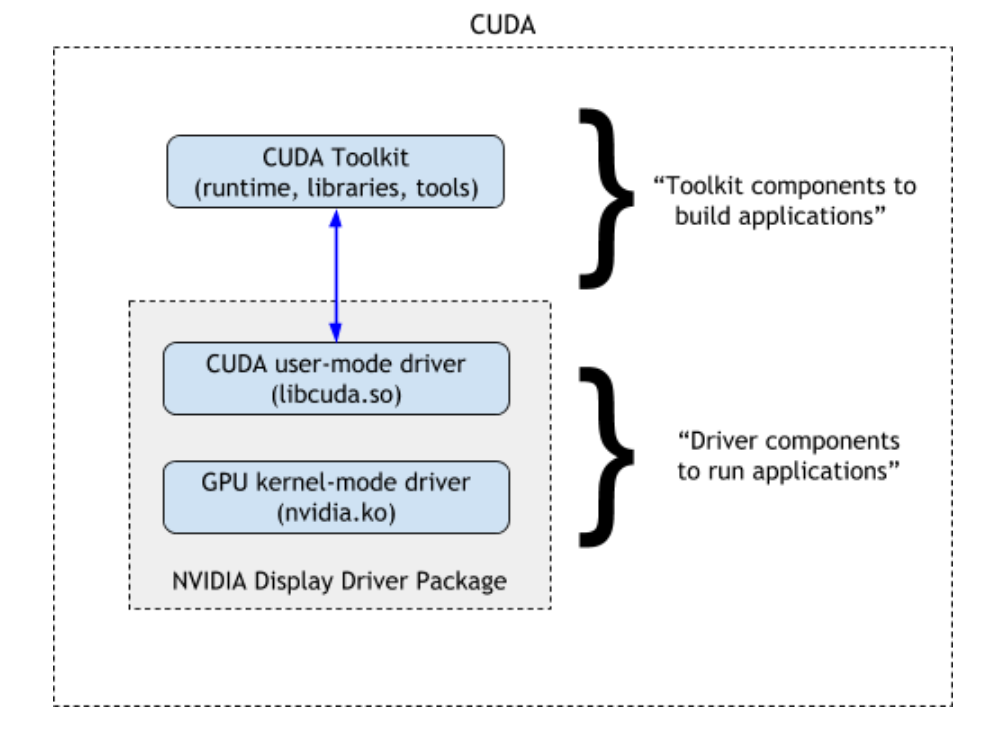
\includegraphics[width=0.75\textwidth]{./img/CUDAcomponents.png}
		   \caption{\small{Schema of the CUDA Components}}
           \end{figure}
     \end{columns}


\end{frame}	

\subsection{Structure of a GPU computation}
\begin{frame}
   \frametitle{Structure of a GPU computation}
      \begin{enumerate}
	 \item \textbf{\textcolor{blue}{Allocate}} memory space on the GPU device.		      
	 \item \textbf{\textcolor{blue}{Transfer}} the data from the CPU to the GPU device. 
	 \item Perform the \textbf{\textcolor{blue}{calculation}} on the GPU device.
            \begin{itemize} 		 
	       \item \textbf{\textcolor{blue}{kernel}}: function executed on the GPU.
               \item To enhance performance: keep data as long as possible on the GPU device.
	    \end{itemize}
         \item \textbf{\textcolor{blue}{Transfer}} the result back from the GPU device to the CPU.
	 \item \textbf{\textcolor{blue}{Deallocate}} memory space on the GPU device.		 
      \end{enumerate}
      \textbf{\textcolor{orange}{Note}}: source code \& makefile available in \texttt{./src}	
\end{frame}


% Allocate & deallocate of GLOBAL memory
\begin{frame}
   \frametitle{Alloc. \& free of global memory on the GPU}
   \begin{itemize}
         \item \lstinline[style=MyCudaStyle]|cudaError\_t| \\
		 CUDA Error types.
	 \item \lstinline[style=MyCudaStyle]|cudaError\_t cudaMalloc(void **devPtr, size\_t size)| \\
		 Allocates memory on the device.
	 \item \lstinline[style=MyCudaStyle]|cudaError\_t cudaFree(void *devPtr)| \\
		 Frees memory on the device.
   \end{itemize}
\end{frame} 

\begin{frame}
   \lstinputlisting[style=MyCudaStyle,basicstyle=\tiny, caption={\texttt{Alloc/Free extract}}]{./latexinc/ex1.cu}
\end{frame}	


% Copy data between host and device
\begin{frame}
   \frametitle{Copy data between host (CPU) and device (GPU)}
       \begin{itemize}
          \item Copy data bewteen host (CPU) and device (CPU) \\		       
                \lstinputlisting[style=MyCudaStyle]{./latexinc/memcpy.cu}
  	  \item Direction (\lstinline[style=MyCudaStyle]|kind|):
             \begin{itemize}
	        \item \lstinline[style=MyCudaStyle]|cudaMemcpyHostToHost|		     
                \item \lstinline[style=MyCudaStyle]|cudaMemcpyHostToDevice|
	        \item \lstinline[style=MyCudaStyle]|cudaMemcpyDeviceToHost|
	        \item \lstinline[style=MyCudaStyle]|cudaMemcpyDeviceToDevice|		
             \end{itemize}			     
       \end{itemize}		  
\end{frame} 

\begin{frame}
   \lstinputlisting[style=MyCudaStyle,basicstyle=\tiny, caption={\texttt{cudaMemcpy extract}}]{./latexinc/ex2.cu}
\end{frame}


% Kernel
\begin{frame}
   \frametitle{CUDA Kernel}
      \begin{itemize}	
	      \item \textbf{\textcolor{blue}{CUDA kernel}}: alias for a function which may run on a GPU device.
	 \item \textbf{\textcolor{blue}{Kernel declaration}} syntax:\\
	       \hspace{6ex}\textit{funcspec} \lstinline[style=MyCudaStyle]|void| \textit{kernelName}(\textit{args})\{ \textit{body} \} \\
               where:
               \begin{itemize}
		  \item \textit{funcspec}: function type qualifier, i.e.\\\lstinline[style=MyCudaStyle]|\_\_global\_\_,\_\_host\_\_,\_\_device\_\_|
                  \item \textit{kernelName}: name of the kernel/CUDA function.
                  \item \textit{args}: argument list of the kernel/CUDA function.
                  \item \textit{body}: body of the kernel/CUDA function (your code).			  
	       \end{itemize}
       \item \textbf{\textcolor{blue}{Kernel call}} syntax:\\
		 \hspace{6ex}\textit{kernelName}\texttt{<<<}\textit{gridSize,blockSize}\texttt{>>>}(\textit{args})\\
               where:
               \begin{itemize}
		  \item \textit{gridSize}: size of the grid of thread blocks.
		  \item \textit{blockSize}: size of a thread block.		       
               \end{itemize}			       
      \end{itemize}
\end{frame}	

% Kernel (Part 2).
\begin{frame}
   \frametitle{Function type qualifiers}
      \begin{table}[H]
	 \begin{center}      
  	    \begin{tabular}{l|l|l}
            Qualifier                                    & Called from  & Executed on   \\
               \hline		
	   \lstinline[style=MyCudaStyle]|\_\_global\_\_| & host         & device\\
 	   \lstinline[style=MyCudaStyle]|\_\_host\_\_|   & host         & host \\
           \lstinline[style=MyCudaStyle]|\_\_device\_\_| & device       & device \\ 
               \hline
            \end{tabular}
         \end{center}
	 \caption{Function type qualifiers}
      \end{table}
      \textbf{\textcolor{orange}{Note:}}\\  	
      \begin{itemize}
         \item You can have to different versions of a function i.e.:\\
	       one with \lstinline[style=MyCudaStyle]|\_\_host\_\_|  \& one with \lstinline[style=MyCudaStyle]|\_\_device\_\_|
      \end{itemize}		      
\end{frame}

% Grid, Blocks and Threads
\begin{frame}
     \frametitle{Grids, Blocks and Threads}
        We have a hierarchical (software) implementation.
     \begin{itemize}
        \item \lstinline[style=MyCudaStyle]|uint3,dim3|:
           \begin{itemize}
              \item CUDA defined structures of unsigned integer \lstinline[style=MyCudaStyle]|x,y,z|
              \item \lstinline[style=MyCudaStyle]|dim3|: based on \lstinline[style=MyCudaStyle]|uint3|
                    but unspecified components are initialized to $1$.
           \end{itemize}
        \item \textbf{\textcolor{blue}{Grid}}: each Grid consists of Blocks
           \begin{itemize}
              \item \lstinline[style=MyCudaStyle]|dim3 gridDim|: dimensions of the Grid.
              \item \lstinline[style=MyCudaStyle]|uint3 blockIdx|: block index within the Grid.
           \end{itemize}
        \item \textbf{\textcolor{blue}{Block}}: each Block consists of Threads
           \begin{itemize}
              \item \lstinline[style=MyCudaStyle]|dim3 blockDim|: dimensions of the Block
              \item \lstinline[style=MyCudaStyle]|uint3 threadIdx|: thread index within the block.
           \end{itemize}
     \end{itemize}
\end{frame}

